
\chapter{Related Work}

Information Retrieval (IR) is a well established research area within
Computer Science.  There are several regular conferences and working
groups on IR topics: ACM SIGIR, TREC, etc.

IR combines the needs for better algorithms for searching, storing, and
displaying data, with aspects of high performance computing and large data
storage.  

\section{Digital Libraries} 
With the growing increase of information globally, the need for better
ways of managing the data are evolving.  Digital Libraries are emerging
which are being investigated to see if they can replace their conventional
counterparts.  One of the main aspects of digital libraries is the loading
of information into the digital library, most of the data is still in
paper format, which has to be converted to digital forms.  Even data
already in digital format may have to be converted into a format suitable
for storage and retrieval.

As said before the amount of data to be stored is ever increasing, in the
order of Gigabytes or even Terabytes are not uncommon.  Storing and
searching through this information is a major task.

The New Zealand Digital Library \cite{www:nzdl} has been a good source of much of the research into the different aspects of IR.

\section{Information Storage}
There are several methods for storing the information, from flat files
stored on file systems to large complex RDBMS.  As well as storing the
actual data, ancillary data, such as indexes, also have to be stored.
The main goal is to allow efficient access to this data.  Although
computers are getting faster and faster, disk accesses still take several
milliseconds.  Hence, one of the main aims is to reduce the number of disk
accesses to retrieve a document.

\section{Indexing Methods}
The main way of retrieving a document is to specify some sort of search
criteria, most often words that appear in the document.  With text
collections of this size, linear searches are not yet possible without
specialist hardware.  Generally some sort of index is needed to narrow the
search space.  These indexes can take several forms:

\subsection{Inverted Indexes}

One of the most popular ways of constructing and index is a structure
called a an \emph{inverted index}.  This is a word-oriented mechanism for
indexing a text collection in order to speed up the searching task. A set
of \emph{inverted lists}, one for each distinct word in the text
collection, is constructed.  It closely resembles the index in the back of
a book, that lists page numbers for each word occurrence.

The index is composed of the \emph{vocabulary} and the \emph{occurrences}.
The vocabulary or lexicon is a list of all distinct words in the text.  For each word
in the vocabulary, a list of document ids, called the \emph{occurrences} is
also stored.

Along with each occurrence, the location of the word in the document may
also be stored.  This aids proximity queries in which the word location is
important.  The \emph{granularity} of the index can vary and each
occurrence may indicate a paragraph, word, or character position.

The space required for the vocabulary storage is a small fraction of the
size of the text.  According to Heaps Law \cite{heaps78}, it grows as
$O(n^\beta)$ where $\beta$ is a constant between 0.4 and 0.6 in practice,
depending on the type of text being stored.

The space required for the occurrences is traditionally $O(n)$, and in
practice is 30 - 40\% of the size of the text collection.  However Witten
et Al \cite{wmb:mg} suggest a compression method that can reduce the size
of the occurrences to just a few percent of the size of the text
collection.  This is discussed further is Section \ref{compression}.

\subsubsection{Index Construction}
Building an inverted index is generally $O(n)$ in complexity, and is a
fairly straight forward task.  The documents are parsed, and each word
occurrence is stored in a tree or hash table.  Each word is searched for in
the tree, if it is found the document number is added to the end of the
word list.  If the word is not found a new node is added to the tree or
hash table, and a new word list started.

Once all the documents have been processed, the index is written to disk.
Each word list is written sequentially to disk, in practise the vocabulary
and occurrences are written to separate files.  The vocabulary file is
normally small enough to be stored in main memory during the query
process, which speeds up searches.  Each word in the vocabulary has a
pointer with it that points the the location of the word list in the
occurrences file.

There are two main problems with this approach -- index size and ease of
updates.  If the document collection is large, then the entire index may
not fit in main memory during construction.  This can be solved by using a
paging mechanism, or compressing the word lists during construction.  The
text collection may be partitioned into smaller sections, each of which is
processed in turn.  The resulting indexes are then merged together.  The
resultant occurrences file cannot be easily updated as it requires
inserting extra word occurrences into the middle of the file.  This is why
most public domain indexers require the entire collection to be re-indexed
after changes to the text collection.  This may be addressed by using a
storage manager of some sort to allow paged updates.

\subsubsection{Searches}
To search the collection, the search terms are first looked up in the
vocabulary.  The word list for each search term is then read from the
occurrences file.  The document ids are read from each word list and are
combined in some way (logical AND, OR, NOT, or some ranked method).

\subsection{Signatures}
Signatures are another word oriented approach to indexing based upon
hashing.  It imposes a smaller, 10 - 20\%, overhead than inverted files,
but requires linear searching.  However the data to be searched in
smaller, and the searching not as complex (bitwise comparisons, rather
than string comparisons).

A hash function creates a bitmap or \emph{signature} of each document (or
text block within a document).  The function maps each word to a bit mask
of $B$ bits.  The signature for the document, is the logical OR of the bit
masks for each word occurring in the document.

Although signatures only return a binary answer to whether a word appears in a document, Croft and Savino propose a ranking method for signatures in \cite{Croft88}.

\subsubsection{Searching}
If a word is present in a document, then the bits set in the words bit
mask, will also be set in the documents signature.  To find a document
containing a set of search terms, a search signature is constructed by
OR'ing all of the search terms.   This search signature is then AND'ed
with each document signature in turn.  The down side of this, is that the
matches may result in false positives.  This is because the hash function
will map more than one word to each possible combination of bits.  Because
of this each match much be verified by a brute force search method to
ensure it is actually a proper match.

\subsubsection{Index Construction}
The construction of the signatures is very simple, for each document, the
bit masks for each word in the document are OR'ed together.  Documents can
be easily added as signatures are simply appended to the end of the
existing ones.  They could even be stored in an RDBMS as a field along
with the text.

This method is actually used in several RDBMS to allow the rapid searching
of large text fields.

\subsection{Suffix Tries}
Inverted indexes and signature files assume the text is composed of words.
This is not always the case, such as in searching through strings of
genetic sequences.

A suffix tree assumes the text is one large string.  Each position in the
text is considered a suffix, that is a string that stretches from that
position to the end of the text.  The start of each suffix is
lexographically different.  Thus, each suffix is then identified by its
position.  Not all text positions need to be indexed, just specific
\emph{index points}, such as word boundaries.  Positions other than these
index points cannot be retrieved (just as in an inverted index, the middle
of a word may not be retrieved).




Each suffix is stored in a tree with pointers to the suffixes stored at
the leaf nodes.  To conserve space the tree is converted into a Patricia
Tree, in which unary paths are compressed into a single node.

The advantage of this method is that phrases are very easy to match, the
disadvantage is the storage requirements are high -- 120 - 240\% of the 
text collection size.

\subsection{Sequential Searching}
Although sequential searching is too slow to cover the entire text, it may
be used in part, once the search space has been narrowed down by other
means.  The details of these methods are beyond the scope of this report,
but include: Brute Force, Knuth-Morris-Pratt, Boyer-Moore, Shift-Or,
and Suffix Automation.      

\section{Compression}
In dealing with such large amounts of data, compression can save large
amounts of storage space.  Not only that, but can often increase
performance too.  Processors and memories are getting faster and faster,
whilst secondary storage is still comparatively slow.  Hence time saved on
reading data from disk can be greater than time taken to decompress it.

\subsection{Text Compression}
There are a variety of means of compressing text which can result in 30 -
70\% space savings. Generally however:

\begin{quote}
The better the compression, the slower the program runs or the more memory
it uses.
\end{quote}

Again the details of the compression methods are out of the scope of this
report, but further details can be found in \cite{witten91indexing,bookstein92model,edleno98:comppatmat,gasieniec99:optlzwpat,navraf99:patzif} and a summary of routines can be found in \cite{wmb:mg}.

One important feature is the synchronisation of the compression methods.
Most compression schemes depend upon previous data, and hence reading
cannot start midway through the compression text.  Synchronisation
points need to be added into the middle of the compression scheme, this is
where the coding is reset to a know state at certain points.  An
alternative is self-synchronising codes, in which the decoder will
automatically come into synchronisation after a while.

Additionally, some interesting work has been done in the above papers on pattern matching in compressed text.  The idea being that a search pattern can be compressed and then matched against the compressed text collection.  This avoids the need to decompress the text first, and also results in less data to actually try the pattern against.

\subsection{Index Compression}
The indexes used to speed up searching can take up a significant
proportion of the overall storage.  By compressing the indexes, the
storage requirements can be reduced, in some cases to the extent that most
of the index can be cached in main memory.  This can prove an enormous
performance gain.

The occurrences in an inverted list are stored in order of document id.
This means that the ids may be represented by the intervals between
successive ids.  These intervals can be stored using fewer bits, hence
less storage.  An upside of this is, the more frequently a word appears,
the smaller the intervals in the word list, and hence the few bits needed
to represent each occurrence.

It is common practice to remove all \emph{stopwords} from the text before
indexing.  These words are frequently occurring words that do not
contribute much to the value of the index.  Articles, prepositions, and
conjunctions are natural candidates for stopwords.  By omitting these
words the index can be reduced by up to 40\%.  In \cite{francis82}, a list of
425 stopwords is presented.


Since these words occur so frequently, their wordlists may be compressed
very effectively.  For example on TREC, the inverted list for the 33 most
common words are stored using just one bit per occurrence, resulting in a
maximum of 741,856 bits long -- about 91KB.  The saving generated by
stopping all 33 words is less than 3MB, which is less than 3\% of the
total 93MB size of the compressed index.

This shows the benefit of eliminating the stopwords before indexing when
using a suitable compression scheme is minimal.  

The workings of the compression schemes are shown in Section
\ref{compression}.

\section{Storage}
\subsection{Index Storage}
The method of storage of indexes on disk is a major factor in the performance of an indexing system.  Using inverted files it is generally not possible to efficiently update the index and insert more data into the middle of the index.  Several papers have been written on how to overcome this problem by using a persistent object store.  This is some method of ensuring the permanence of objects in memory.  Brown et Al \cite{ncstrl.umassa_cs//UM-CS-1993-067} describe the way they took an existing information retrieval system, INQUERY, and replaced its custom data management system with a persistent object store, Mneme \cite{Moss:1990:DMP}.  Their positive results showed that this may be an area worth looking into in greater depth in the future.

\subsection{Updating Indexes}
Most IR systems do not support the addition of new documents to the indexes due to the problems outlined above.  However modern applications like OSDigger or News filters work in a dynamic environment and require frequent updates of the indexes.  Tomasic \cite{Tomasic:1994:IUI} describes a method of overcoming this problem by using a dual-structure index.  Words that are very common are stored in a different structure to those that are not so common.  This allows different policies to be employed as to how the indexes are updated.  Using persistent object stores as described above, Brown et Al \cite{vldb:BCC94} further show that using persistent object stores abstracts the need for special treatment of updating indexes.  Their experimental results show much improved performance over traditional methods of updating indexes.

\subsection{Distributed Searches}
Research has been done into using networks of computers to run in parallel for Information Retrieval.  The extra power and memory of using multiple computers can speed up both the indexing process and also the query process.  The main area of research is how to efficiently break the task up into subtasks to be executed in parallel.  The methods used in the OSDigger system increase the efficiency of the indexing and searching to a point where the tasks can be run on a single computer.  Stanfill, Thau and Waltz describe an algorithm for constructing indexes in parallel in \cite{Stanfill89}.  Lu and McKinley describe a method of searching a terabyte of text using partial replication on a large parallel computer in \cite{luMcK:Search_tera_repli}.  Large web search engines such as AltaVista and Infoseek handle their enormous loads by using large farms of machines in parallel.  The overhead of communication and synchronisation to get the whole system to function may actually degrade performance as described by Lu, McKinley and Cahoon in further work \cite{zhihong98:_hardw_softw_balan_act_infor}.


\section{Algorithms}
\subsection{Compression Schemes}
\label{compression}

The inverted file compression plays a large part of this project and is
what enables the search system to perform so well on modest hardware.
Firstly, an inverted index is composed of an inverted list for each word
that occurs in the lexicon.  Suppose a term $t$ appears in five documents,
those numbered 3,5,20,21,76.  This term is represented in the index by a
list:

\[
\langle 5;3,5,20,21,76 \rangle
\]

The offset of this list in the inverted file is often stored in the
lexicon, so that the list can be found without searching.  In general the
list is of the form:

\[
\langle f_t;d_1,d_2,d_3,...,d_{f_t} \rangle 
\]

Since the list of document numbers is in ascending order the document
numbers could be represented by the intervals, or \emph{d-gaps}, between
each successive document number.  Hence the previous list becomes:

\[
\langle 5;3,2,15,1,50 \rangle 
\]

The original document numbers can be re-constructed by calculating the
cumulative sums of the d-gaps.

Although the largest d-gap is still of the same magnitude as the original
list, the distribution of numbers has changed.  There will be far more
smaller numbers than before.  This is especially so for frequent words
which will have more entries, each of a smaller d-gap.

Specific models have been developed to take advantage of this shift in
probability distribution.  They can be roughly grouped into two classes:
\emph{global} methods, in which each list is encoded with the same
parameters, and \emph{local} methods which use different encoding
parameters for each list, depending upon the values being coded.  A list of some of these models is shown in Table \ref{models}. In
general local methods will always outperform global methods, and they are
not any more computationally expensive, but maybe slight more complicated
to implement.  Of the local methods, the most suitable for general text is
the Local Bernoulli Method, using Golomb coding.  As this is the actual coding method used in the final project, it will be explained here.


\begin{table}[t]
\begin{center}
\begin{tabular}{ll}
Method & Reference \\
\hline
\emph{Global Methods} \\
\hspace{5mm} \emph{Nonparameterized} \\
\hspace{10mm} Unary \\
\hspace{10mm} Binary \\
\hspace{10mm} $\gamma$  & \cite{elias75universal,bentley76} \\
\hspace{10mm} $\delta$ & \cite{elias75universal,bentley76} \\

\hspace{5mm} \emph{Parameterised} \\
\hspace{10mm} Bernoulli & \cite{gallager75optimal,golomb66} \\
\hspace{10mm} Observed frequency \\

\hline

\emph{Local Methods} \\
\hspace{5mm} Bernoulli & \cite{witten91indexing,bookstein92model} \\
\hspace{5mm} Skewed Bernoulli & \cite{teuhola78,moffat92param} \\
\hspace{5mm} Hyperbolic &  \cite{schuegraf76} \\
\hspace{5mm} Observed frequency  \\
\hspace{5mm} Batched frequency & \cite{moffat92param}\\
\hspace{5mm} Interpolative   \\

\end{tabular}
\caption{Some methods for compressing inverted files}
\label{models}
\end{center}
\end{table}

\begin{table}[htbp]
  \begin{center}
    \begin{tabular}{llllll}
      Gap $x$ & \multicolumn{5}{c}{Coding Method} \\
      \cline{2-6} 
            & Unary & $\gamma$  & $\delta$ & \multicolumn{2}{c}{Golomb} \\
            \cline{5-6}
            &       &           &          &  $b = 3$ & $b = 6$  \\
      \hline
        1       &       0               &       0       &       0               &       00      &       000 \\
        2       &       10              &       100     &       1000            &       010     &       001 \\
        3       &       110             &       101     &       1001            &       011     &       0100 \\
        4       &       1110            &       11000   &       10100           &       100     &       0101 \\
        5       &       11110           &       11001   &       10101           &       1010    &       0110 \\
        6       &       111110          &       11010   &       10110           &       1011    &       0111 \\
        7       &       1111110         &       11011   &       10111           &       1100    &       1000 \\
        8       &       11111110        &       1110000 &       11000000        &       11010   &       1001 \\
        9       &       111111110       &       1110001 &       11000001        &       11011   &       10100 \\
        10      &       1111111110      &       1110010 &       11000010        &       11100   &       10101 \\
    \end{tabular}
    \caption{Example codes for integers}
    \label{tab:codes}
  \end{center}
\end{table}

\subsubsection{Golomb Coding}
This method was first described by Solomon Golomb in 1966 \cite{golomb66}.  For some parameter $b$ any number $x > 0$ is coded in two parts: first, $q + 1$ in unary, where the quotient $q = \left\lfloor \frac{(x - 1)}{b}\right\rfloor$.  The remainder $r = x - qb - 1$ is coded in binary, requiring $\log b$ bits.

For example, with $b = 3$ there are three possible remainders $r=0...2$, coded 0, 10 and 11, respectively.  Similarly for $b = 6$ there are six possible remainders $r = 0...5$, coded 0, 01, 100, 101, 110, and 111, respectively.  If the value $x = 9$ is to be coded with $b = 3$, calculation gives: $q=2$ and $r=2$ because $9-1 = 2\times3+2$.  Thus, the encoding is 110 followed by 11.  If coded with $b=3$, the values calculated are $q=1$ and $r=2$, resulting in the encoding 10 followed by 100.  Other codings for small values of $x$ can be seen in Table \ref{tab:codes}.

Gallager and Van Voorhis \cite{gallager75optimal} showed that if $b$ is chosen to satisfy

\[
(1-p)^b + (1-p)^{b+1} \leq 1 \leq (1-p)^{b-1} + (1-p)^b
\]

this coding generates an optimal prefix-free code for the geometric distribution corresponding to Bernoulli trials with the probability of success given by $p$.

Witten et al \cite{wmb:mg} show that assuming, $p = \frac{f}{N \times n} \ll 1$, a useful simplification is

\[
b^A \approx \frac{\log_e 2}{p} \approx 0.69 \times \frac{N \times n}{f}
\]

Where $N$ is the total number of documents, $n$ is the number of distinct terms, and $f$ is the number of index pointers.

\subsubsection{Local Bernoulli Model}
The value of $b$ described above is calculated from the statistics of the entire text collection.  However some words are more common than others, in which case their word lists will contain many more terms in them with much smaller d-gaps.

If the frequency, $f_t$, of term $t$, is known, then a Bernoulli model on each individual list can be used.  Using this method, frequent words are encoded with a smaller value of $b$ than infrequent words.  Very common words are encoded with $b=1$ which causes the code to degenerate to a set of unary codes for the gap sizes with no binary components.  This is equivalent to storing the word list as a \emph{bitvector}, which is a binary vector in which each document is represented by a bit, the bit being set if the word appears in that document.

For frequent words, this can result in a word list compressed to just 3-4\% of its original size, compared to storing each document number as an uncompressed 32-bit integer.

\subsection{Document Ranking}

Once the index has been constructed and a query is issued to be tried on the index, the outcome is a set of documents that somehow match the query terms.  In order to determine what is matched and what is not (and to what degree it matches) a similarity measure is needed.

\subsubsection{Boolean Queries}
These queries are the simplest to implement.  Either a term appears in a document or it does not.  A term is constructed of a set of queries terms with some logical operators eg. FreeBSD \emph{and} scsi, linux \emph{or} FreeBSD, linux \emph{not} debian.  These terms are matched against the index and matching documents are returned in no particular order.

\subsubsection{Ranked Queries}
These queries are more complicated, they order the resultant set of documents in some order with the most likely candidates at the top of the results.  This is intuitively how mast users expect a search system to work.  However, how does the search system determine how \emph{relevant} a document is?  This has been studied in great depth and a number of methods have emerged.  The details of each of these methods is beyond the scope of this report, however some of them are listed with references in Table \ref{tab:methods}

\begin{table}[htbp]
  \begin{center}
    \begin{tabular}{ll}
      Model & Reference \\
      \hline
      \emph{Classic Models} \\
      \hspace{5mm} Boolean Model & \cite{wmb:mg,BasRib} \\
      \hspace{5mm} Vector Model & \cite{salton71,salton68} \\
      \hspace{5mm} Probabilistic Model & \cite{robertson76,fuhr92} \\
      \emph{Alternative Set Theoretic Models} \\
      \hspace{5mm} Fuzzy Set Model & \cite{radecki79} \\
      \hspace{5mm} Extended Boolean Model & \cite{salton83} \\
      \emph{Alternative Algebraic Models} \\
      \hspace{5mm} Generalised Vector Space Model & \cite{wong85} \\
      \hspace{5mm} Latent Semantic Indexing Model & \cite{furnas88,hull94} \\
      \hspace{5mm} Neural Network Model & \cite{wilkinson91} \\
      \emph{Alternative Probabilistic Models} \\
      \hspace{5mm} Bayesian Networks & \cite{pearl88,fung95} \\
      \hspace{5mm} Inference Network Model & \cite{turtle91,turtle90,LuCallanCroft91:infer_nets} \\
      \hspace{5mm} Belief Network Model & \cite{ribeiro96} \\
    \end{tabular}
    \caption{Ranking Models}
    \label{tab:methods}
  \end{center}
\end{table}

Each of these methods has its good and bad points, and as always a trade-off between complexity, processing speed, and accuracy.


\subsubsection{Document and Term Weights}
When trying to rank documents one of the main problems is trying to work out how relevant a document is to a query.  The main intuitive way of thinking of this, is that a document that contains more occurrence of the query term is more important than one that contains less.  However, what happens when a query consists of several terms? Should each term have the same \emph{weight} in the query?  If the query \emph{java database} was issued, should a document that mentions \emph{java} lots of times, but \emph{database} only once, be ranked more or less relevant than one than mentions \emph{database} many times and \emph{software} only once?  What is needed is some way of determining the usefulness or weight of each term in a document (or query).

George Zipf noted in his book \emph{Human Behaviour and the Principle of Least Effort} \cite{zipf49} that the frequency of an item tends to be inversely proportional to its rank.  That is, the weight $w_t$ of a term $t$ might be calculated as:

\[
w_t = \frac{1}{f_t}
\]

where $f_t$ is the frequency of the term in the text collection.

This can be combined with a \emph{relative term frequency}, denoted $r_{d,t}$ to give the document-term weight $w_{d,t}$ and/or the query-term weight $w_{q,t}$.

Other methods of calculating $w_t$ are mentioned in \cite{wmb:mg} however the most usual is

\[
w_t = \log_e \left( 1 + \frac{N}{f_t}\right)
\]

where $N$ is the number of documents in the collection.  The logarithm is added to prevent a term with $f_t =1$ from being regarded as twice as important as $f_t = 2$.

The relative term frequency factor, $r_{d,t}$ can also be calculated in several ways, the most usual being

\[
r_{d,t} = 1 + \log_e f_{d,t}
\]

The logarithm here prevents the number of occurrences of the term in a document from contributing too much as the number of occurrences increase.

The document vectors can then be calculated as:

\[
w_{d,t} = r_{d,t} \cdot w_t
\]

These style of weightings are loosely known as TD $\times$ IDF, term frequency times inverse document frequency, and play an important part of search ranking.

\subsubsection{Cosine Measure}
The ranking system used in OSDigger is a vector space model known as the Cosine Measure.

Each document is represented as an vector in $n$-dimensional space in which each dimension represents a different term in our lexicon.  If we also represent the query terms in this fashion, as a vector, then the similarity between the two is proportional to the similarity in direction of the two vectors.

This is a well understood concept in vector algebra -- it is the angle between the two vectors.  Simple algebra yields:

\[
X \cdot Y = |X| |Y| \cos \theta
\]

where $X \cdot Y$ is the vector inner product and

\[
|X| = \sqrt{\sum^n_{i=1} x^2_i}
\]

is the Euclidean length of $X$.  The angle $\theta$ can be calculated from

\[
\cos \theta = \frac{X \cdot Y}{|X| |Y|} = \frac{\sum^n_{i=1} x_i y_i}{\sqrt{\sum^n_{i=1} x^2_i} \sqrt{\sum^n_{i=1} y^2_i}}
\]

This makes sense as by dividing by the Euclidean length of the vectors we normalise their lengths.  This removes the effect of the length of the document, in that long documents are not favoured over shorter ones.

If the documents are each vectors in the positive region of an $n$-dimensional space, then the query term can be imagined as a ray that emanates from the origin in a particular direction.  The document vectors that lay closest to the this ray in an angular sense are the most relevant.

This leads to the \emph{cosine rule} for ranking

\begin{eqnarray*}
  \textrm{cosine}(Q,D_d) & = & \frac{Q \cdot D_d}{|Q| \cdot |D_d|} \\
                         & = & \frac{1}{W_q W_d}\sum^n_{t=1} w_{q,t} \cdot w_{d,t} \\
\end{eqnarray*}

where
\[
W_d = \sqrt{\sum^n_{t=1} w^2_{d,t}}
\]

is the Euclidean length -- ie. the \emph{weight} -- of document d and

\[
W_q = \sqrt{\sum^n_{t=1} w^2_{q,t}}
\]

is the weight of the query.

\chapter{Technical Basis}
\label{techbasis}


\section{OSDigger Implementation}
As seen in the previous chapter there are lots of possible methods of indexing and searching, below is presented the technologies and algorithms that OSDigger uses and why.

\subsection{Storage}
The storage of the messages themselves and the storage of the indexes are two different matters.  Although it is possible that they could both be stored in the same manner, this would not be optimal for either of them.

The messages are stored in MySQL, an Open Source RDBMS \footnote{Relational Database Management System}.  This was chosen as it allows very fast read access to the data, and allows storage of large objects.  MySQL does not support server-side procedures or fine-grained locking as Oracle or PostgreSQL \cite{www:postgresql} do, but these features are not that important for this application.  MySQL does support user defined functions (UDFs) that can be written in C and could be used to perform task such as on-the-fly compression/decompression or parsing of a field.  An RDBMS was used so that various headers in the messages could be stored as separate fields in the database and searched on in a relational way. eg. Find all messages last year from Jordan Hubbard on the FreeBSD Questions list.

Several methods were investigated for storing the indexes.  Initially for the prototype the indexes were stored as a binary file to disk in some manner.  The indexer and search programs knew how to handle the files internally.  One of the main problems with this approach was managing concurrent access, and how to find a particular inverted list in the inverted file.  Initially when the inverted file was written to disk, a second file -- an index was also written.  This listed the offsets of the word lists for each word in the inverted file.  This still did not address the concurrency issue.

Several persistent object stores were looked at: Generic Object Oriented Database System (GOODS) and Persistent Object Storage for C++ (POST++) \cite{www:goods} , both written by Konstantin Knizhnik of the DEC Moscow Software Center, however both required either C++ or Java knowledge which I did not have at the time of reviewing them.  If more time was available I would like to have investigated these further as previous research into using Persistent Object Stores has been optimistic.  

In the end the BerkeleyDB \cite{olson99,www:berkeleydb} embedded database was used.  This is a key/value pair database, that provides exceptional speed, and is simple to integrate.  It has no arbitrary record limits, so scales to the size needed.  The DB supports B+tree, Extended Linear Hashing, Fixed and variable-length records, all with the same interface.  It also has caching, locking and transactional subsystems.

\subsection{Word Stemming}
Before words in the documents are indexed, the suffixes are removed, this is known as \emph{stemming.}  This is to reduce the number of different variations of a word.  As an effect of this it normally reduces words to a single tense. eg. \emph{run}, \emph{runs}, \emph{running} are all reduced to \emph{run}.

There are several stemming algorithms around, the two most common are the Porter stemming algorithm \cite{porter80} and the Iterative Lovins algorithm \cite{lovins68}.  A comparison of these and other algorithms are are detailed in \cite{frakes-stemming}.

Due to its simplicity OSDigger uses Porters algorithm.

\subsection{Index Compression}
The indexes are compressed using the Local Bernoulli model with Golomb Coding, as described in Section \ref{compression}.  This scheme turned to to be extremely fast and the indexes used in the prototype were compressed to just over 4 bits per pointer.

\subsection{Index Construction}
There are two methods of dealing with updating indexes: Creating a dynamic index structure that can be expanded, or re-indexing the entire collection.  The former traditionally takes too long to be done very often, and the latter requires complex data structures and better underlying storage management.

Profiling the prototype indexer highlighted an important fact.  The majority of the time spent constructing the index, is actually spent parsing the documents and stemming the words.  Hence if the index was going to be rebuilt from scratch each time it would take quite a while.  To solve this an intermediate \emph{forward} index is needed.  This index is not inverted and so can be appended to when new documents arrive.  The inversion of this index is very efficient as there is no parsing or stemming to do.

\begin{quote}
  This gives us a unique hybrid approach to updating the indexes.  The
  forward index is incrementally updated; and the inverted index can
  be re-created very often as it can be constructed quickly from the
  forward index.
\end{quote}

The indexes are constructed in two phases.  First the documents are extracted from the MySQL database and parsed.  Each word is looked up in a lexicon (stored in a BerkeleyDB), and a new wordid is assigned if the word does not yet exist in the lexicon.  A forward index is constructed which details words are in a document.  This is stored compressed.  Each list is then stored in a BerkeleyDB with the document number as a key.  Note: this has not yet been inverted.  It is just a more efficient representation of what is in the messages.

\begin{figure}[htbp]
  \begin{center}
    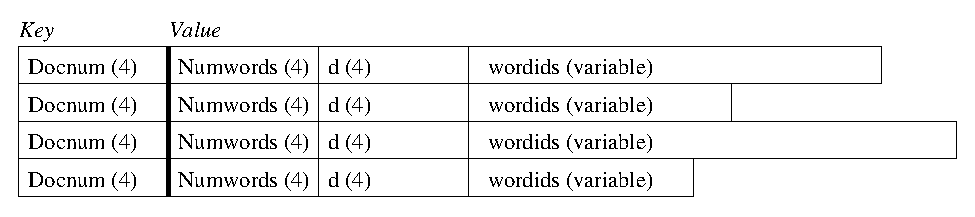
\epsfig{file=figures/forward.eps,width=12cm}
    \caption{Format of Forward Index}
    \label{fig:forward}
  \end{center}
\end{figure}

The format of the forward index can be seen in Figure \ref{fig:forward}.  The numbers in parenthesis are the length of each field in bytes. \emph{D} is the local Bernoulli parameter used to encode and decode that list, \emph{Numwords} is the number of words encoded in that list.

The forward index is actually partitioned into multiple indexes.  Each index contains a subset of the total terms in the lexicon.  A hash value is used to calculate which word goes in which index.  This results in several entries for each document, each in a different index.  This adds a slight bit to the overhead, but means that then terms are now partially ordered.  This concept was taken from the method used for the indexes of Google \cite{Brin+Page+1998a}, a large web search engine.

An inverted index is create from each forward index.  This results in each inverted index containing complete lists for for a subset of the words.  The reason for doing this, is that each forward index can be processed independently, requiring less memory.   The inverted indexes are a similar format to the forward indexes and is shown in Figure \ref{fig:inverted}.  The inverted indexes are again stored in a BerkeleyDB database with the wordid as the key.

\begin{figure}[htbp]
  \begin{center}
    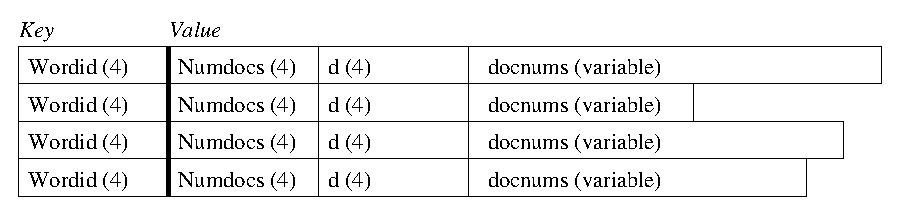
\epsfig{file=figures/inverted.eps,width=12cm}
    \caption{Format of Inverted Index}
    \label{fig:inverted}
  \end{center}
\end{figure}



\subsection{Searches}
Two searching methods are supported by OSDigger:
\subsubsection{Onestep Searches}
The Onestep search works like most other search engines in that the user enters a set of search terms and a list of documents are returned.


\subsubsection{Twostep Searches}
The Twostep search tries to overcome the main problem of searching -- the user.  Often a user does not exactly know what they are searching for and prefer to enter in a couple of terms and then look at the results.  They then refine their query, adding terms the saw from the first search and try again.  Research shows that he average user enters only 2 query terms on average.  There is no way a search engine can determine exactly what a user is looking for with just 2 terms. eg. a child entering in \emph{dinosour food} will most likely be looking for something entirely different to a paleontologist entering in \emph{dinosaur food}.  The only way a search engine can return the correct results is to somehow get more information from the user as to what they are searching for.  Often this is done by presenting the user with a set of sample documents and asking them to indicate which are most like what they are looking for.  The search process is the re-iterated.

OSDigger supports another method.  With the Twostep search a user enters in their query as normal, but instead of presented with the results, they are presented with a list of additional query terms related to what they first entered.  This is to encourage the user to enter in more terms.  Even if none of the terms presented are exactly what they had in mind, they may jog the user into thinking more about specific terms to aid the query.

The process works by looking into the forward indexes created by the indexer, and making note of all the words that have appear in the top 15 documents returned by the Onestep process.  Each word is then looked up in the lexicon to find out the total number of times it occurs.  Using this information a TD $\times$ IDF score can be computed for each word.  Any word which appears often in the set of results relative to how often it appears in the entire text collection is considered a related word and is returned.

Results show this method in many cases to be quite effective.  Results from the query \emph{FreeBSD sound card} are shown in Table \ref{tab:twostep}

\begin{table}[htbp]
  \begin{center}
    \begin{tabular}{|l|l|l|l|l|}
      \hline
      Score & Wordlog & $F$ & $f$ & word \\
      \hline
      \hline
22.70   &       6.61    &       1944    &       30      &       sound\\
17.69   &       5.64    &       4011    &       22      &       card\\
16.90   &       9.43    &       63      &       5       &       blaster\\
16.72   &       6.97    &       1424    &       10      &       3.1\\
15.40   &       7.91    &       558     &       6       &       pnp\\
15.17   &       8.46    &       291     &       5       &       oss\\
14.74   &       9.16    &       105     &       4       &       theme\\
14.58   &       6.33    &       2429    &       9       &       pci\\
14.54   &       7.47    &       875     &       6       &       dwhite\\
13.16   &       8.17    &       414     &       4       &       128\\
13.14   &       3.76    &       12917   &       32      &       freebsd\\
13.04   &       9.41    &       66      &       3       &       ess\\
12.68   &       9.14    &       108     &       3       &       soundcard\\
12.58   &       9.08    &       121     &       3       &       pcm0\\
12.51   &       9.03    &       131     &       3       &       snd0\\
12.40   &       5.64    &       4150    &       8       &       driver\\
12.37   &       5.37    &       4883    &       9       &       under\\
12.26   &       8.84    &       174     &       3       &       x11amp\\
12.19   &       8.79    &       188     &       3       &       maker\\
12.14   &       8.76    &       197     &       3       &       soundblaster\\
\hline
    \end{tabular}
    \caption{Twostep results for \emph{freebsd sound card}}
    \label{tab:twostep}
  \end{center}
\end{table}

where \emph{Score} is how relevant a word is, \emph{Wordlog} is the TD $\times$ IDF for that word, $F$ is how often that word appears throughout the collection and $f$ is how often the word appeared in the top 15 documents returned by the Onestep query.

As expected \emph{sound} and \emph{card} are near the top as they are the actual search terms.  Other notable terms are \emph{blaster} coming from Sound Blaster a make of sound card; \emph{oss} the Open Sound System; \emph{pcm0} and \emph{snd0} are audio devices under unix; \emph{x11amp} is an audio player application; \emph{soundcard} and \emph{soundblaster} are variations on above.

\section{User Interface}
\label{sec:ui}
One of the main goals of software engineers is to separate the logic and the presentation of a system.  To this end we have decided to use Extensible Markup Language (XML) \cite{www:xml} to pass the data from the search server to the web server for presentation to the user.  A java servlet running on the web server then applies an Extensible Style Sheet Transformation (XSLT) \cite{www:xslt} to the XML data to convert it into the HTML page.

This has the advantage of separating the logic and the presentation in such a way that a web designer can work on the layout of the web site, whilst a software engineer can work on the backend search server.

A very simple example of an XSLT transformation is shown below.  Assume we had some XML document representing a business card:

\begin{verbatim}
  <card type="simple">
    <name>John Doe</name>
    <title>CEO, Widget Inc.</title>
    <email>john.doe@widget.com</email>
    <phone>(202) 456-1414</phone>
  </card>
\end{verbatim}


We define the XHTML\footnote{A well-formed XML version of HTML} rendering semantics for our business-card markup language using an XSLT stylesheet: 

\begin{verbatim}
  <xsl:stylesheet xmlns:xsl="http://www.w3.org/XSL/Transform"
                  xmlns="http://www.w3.org/1999/xhtml">
  <xsl:output doctype-system=
       "http://www.w3.org/TR/xhtml1/DTD/xhtml1-transitional.dtd"/>
  
    <xsl:template match="card[@type='simple']">
      <html xmlns="http://www.w3.org/1999/xhtml">
        <title>business card</title><body>
          <xsl:apply-templates select="name"/>
          <xsl:apply-templates select="title"/>
          <xsl:apply-templates select="email"/>
          <xsl:apply-templates select="phone"/>
      </body></html>
    </xsl:template>
  
    <xsl:template match="card/name">
      <h1><xsl:value-of select="text()"/></h1>
    </xsl:template>
  
    <xsl:template match="email">
      <p>email: <a href="mailto:{text()}"><tt>
        <xsl:value-of select="text()"/>
      </tt></a></p>
    </xsl:template> 

    ...
  </xsl:stylesheet>
\end{verbatim}

After combining the two we get the resulting XHTML document: 

\begin{verbatim}
  <!DOCTYPE html SYSTEM 
     "http://www.w3.org/TR/xhtml1/DTD/xhtml1-transitional.dtd">
  <html xmlns="http://www.w3.org/1999/xhtml">
  <title>business card</title>
  <body><h1>John Doe</h1><h3><i>CEO, Widget Inc.</i></h3>
  <p>email: <a href="mailto:john.doe@widget.com">
  <tt>john.doe@widget.com</tt></a></p>
  <p>phone: (202) 456-1414</p>
  </body></html>
\end{verbatim}

which a web browser might display like:

\begin{center}
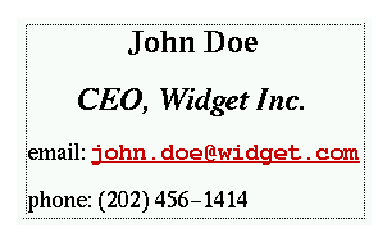
\epsfig{file=figures/xmlex.eps,width=6cm}
\end{center}

This also allows us to easily construct multiple front ends for the site.  These could be different HTML styles, eg. a low bandwidth version with less graphics, or even another XML format, such as WML\footnote{Wireless Markup Language} for use on WAP\footnote{Wireless Application Protocol} mobile phones and handheld PCs.

% LocalWords:  SIGIR TREC Terabytes RDBMS ids Witten Savino OR'ing AND'ed OR'ed
% LocalWords:  lexographically stopwords wordlists KB MB INQUERY Mneme OSDigger
% LocalWords:  Tomasic Stanfill Thau Lu terabyte AltaVista Infoseek Cahoon htbp
% LocalWords:  Golomb Nonparameterized Gallager Voorhis al bitvector eg scsi TD
% LocalWords:  linux debian Zipf IDF MySQL PostgreSQL UDFs Konstantin Knizhnik
% LocalWords:  Center BerkeleyDB Lovins wordid eps Numwords Google Onestep pnp
% LocalWords:  Twostep dinosour Wordlog oss pci dwhite freebsd ess soundcard TR
% LocalWords:  pcm snd soundblaster unix XML servlet XSLT HTML XHTML stylesheet
% LocalWords:  xsl xmlns http www org xhtml doctype DTD dtd html href mailto tt
% LocalWords:  xmlex WML WAP handheld
